
\documentclass{beamer}

\usepackage{default}
\setlength{\leftmargini}{0pt}

\title{Rube Goldberg Machine: \\CS251 Project by Group 02}
\author{Harshal ,  Tanmay, \quad Navneet\\140050003  140100011  140100090\\ harshal.m \quad  tanmayb \quad navneet}
\institute{IIT Bombay}


\begin{document}
\maketitle
\begin{frame}{Introduction}
\begin{center}
\textbf{\Large{Water Server}}
\end{center}
\begin{itemize}[label = {}]
\item[]<1-> What is a Rube Goldberg Machine?
\item[]<2-> A Rube Goldberg machine is a contraption, invention, device or apparatus that is deliberately over-engineered to perform a simple task in a complicated fashion, usually including a chain reaction.\textit{\tiny{\{Reference: Wikipedia\}}}
\item[]<3->Water Server (:P): Serves water from two containers into a glass placed originally at adifferent location
\end{itemize}
\end{frame}

\begin{frame}{Key Components}
\begin{minipage}[t]{0.48\linewidth}
\begin{enumerate}
\item<1-> Dominos
\item<1-> Pulleys
\item<2-> Snooker table
\item<2->Conveyor Belt
\item<3->Newton's Cradle
\item<4->Mills
\item<5->Fluid
\item<6->Criss-cross structure
\end{enumerate}
\end{minipage}
\begin{minipage}[t]{0.48\linewidth}
\hfill \break
\begin{itemize}
\item[]<7-> 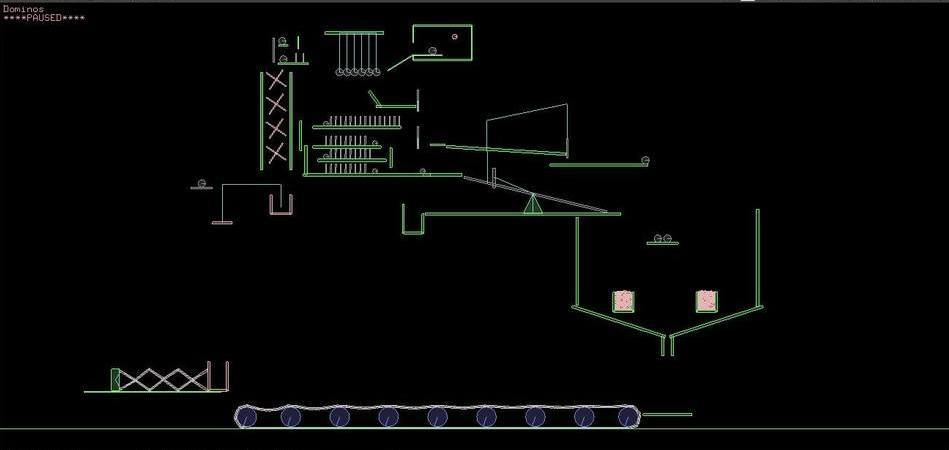
\includegraphics[width=5cm]{img/whole}
\end{itemize}
\end{minipage}
\end{frame}
\begin{frame}{Working}
\begin{itemize}[leftmargin=]
\item[]<1-> \textbf{Initialization}
\begin{itemize}
\item<2-> A snooker ball on the table hits the three sides of the walls finally just bruising the ball giving it enough velocity to initialize the system.
\end{itemize}
\item[]<3-> \textbf{Setup for Container}
\begin{itemize}
\item<4-> The ball hits the Newtons Cradle which starts a small sequence of Dominos present on the left
\item<4-> The dominos hits the ball which hits the vertical plank before falling into the mill causing the second ball to fall into the mill as well
\item<5-> The balls fall into the open box which tips the horizontal plank on its downward movement. The heavy ball on the horizontal plank falls on the criss cross structure and the container is pushed on the conveyor belt below
\end{itemize}
\end{itemize}
\end{frame}
\begin{frame}{Working}
\begin{itemize}
\item[] \textbf{Setup for Pouring Water}
\begin{itemize}
\item<2-> The ball which hits the Newton's Cradle falls down and initializes many sequences of the multi-level dominos sequence
\item<2-> The ball later gets obstructed by the gate.
\item<3-> The dominos will push the balls onto the seasaw which will initialize the gate at which the ball from the Newton's Cradle was held.  
\item<4-> The ball hits another ball tipping it over and later pushes the two balls into the container containing water
\item<5-> The overflown water falls into the funnel, which is later collected into the vessel
\end{itemize}
\begin{center}
\item[]<6-> \huge{Thank You!}
\end{center}
\end{itemize}
\end{frame}
\end{document}
